% Provenance (never printed): see sources/outline_sources.md (Year 2: ore deposits ---
% magmatic, hydrothermal, sedimentary and supergene deposits; grade and tonnage; exploration).
% Deposit descriptions from the USGS Mineral Deposit Models for Resource Assessment
% (Scientific Investigations Report 2010-5070, chapters A, B, C, E, I, L, N, O, Q), USGS
% Open-File Report 03-077 (orogenic gold) and Grabreck et al. 2022 (kimberlites); the grade and
% tonnage data of the world's porphyry copper deposits from USGS Open-File Report 2008-1155
% (dataset bachelor-2-porphyry-cu). Ledger rows in sources/ledger/book4.md; curves and numbers
% from figdata/bachelor-2/ores.py and the Book 4 second-writer scratch calculator calc/ch29.py.
% Geology and sourced numbers only: no advocacy.
\chapter{Ore Deposits}\label{ch:b2:ore-deposits}

Copper makes up about \qty{0.006}{\percent} of the crust; it is mined from rock that holds about
\qty{0.5}{\percent}. Every copper mine therefore sits on rock some eighty times richer than the
crust around it, and every \omterm{def:b2:ore-deposits:deposit}{ore deposit} is the work of a natural concentrator: a \omterm{def:b2:magma-emplacement:magma}{magma} that
unmixed a sulfide liquid, a hot brine that dissolved metals and dropped them in a fracture, a
river that sorted heavy grains from light ones, rain that leached the top of an orebody and
redeposited its copper below. This chapter follows these concentrators, then measures their
products --- how much ore, at what grade --- and ends with the way deposits are found.
% ledger: perkins:ore-grades

\begin{recall}
\textbf{From the school volumes}: \omterm{def:b2:ore-deposits:deposit}{ore deposit} and \omterm{def:b2:ore-deposits:cf}{concentration factor}, vein, \omterm{def:b2:ore-deposits:placer}{placer}, reserve and
resource; hydrothermal circulation and black smokers at ridges. \textbf{From the chemistry
books}: ore; solubility, complex ions and redox. \textbf{From the Year 1 volume}: the settling
velocity of a grain and Stokes's law; laterite; evaporite. \textbf{From
\cref{ch:b2:elements-in-the-earth}}: \omterm{def:b2:elements-in-the-earth:goldschmidt}{chalcophile element}, the \omterm{def:b2:elements-in-the-earth:partition}{mineral--melt partition
coefficient}. \textbf{From \cref{ch:b2:magmatic-differentiation}}: \omterm{def:b2:magmatic-differentiation:cumulate}{layered intrusion} and
\omterm{def:b2:magmatic-differentiation:cumulate}{cumulate}. \textbf{From \cref{ch:b2:precambrian-earth}}: \omterm{def:b2:precambrian-earth:bif}{banded iron formation}, \omterm{def:b2:precambrian-earth:craton}{craton}.
\textbf{From the mathematics books}: the normal and log-normal distributions, and the normal
distribution function $\Phi$.
\end{recall}

\section{Ore, grade and concentration}\label{sec:b2:ore-deposits:grade}

\begin{definition}[Gangue]\label{def:b2:ore-deposits:ore}
In an ore, the \emph{gangue}\index{gangue} is everything that has no economic value: the
rock-forming, hydrothermal and weathering minerals that accompany the ore minerals and are
separated from them and discarded during processing.
\end{definition}

Most ore is \omterm{def:b2:ore-deposits:ore}{gangue}. In a \omterm{def:b2:ore-deposits:hydrothermal}{porphyry copper deposit}, the world's main source of copper, more than
\qty{98}{\percent} of the ore is \omterm{def:b2:ore-deposits:ore}{gangue}, and the copper minerals make up the rest.
% ledger: usgs10b:share

\begin{definition}[Ore grade, cut-off grade, tonnage]\label{def:b2:ore-deposits:grade}
The \emph{ore grade}\index{ore grade} of a volume of rock is the mass fraction of the valuable
element or mineral in it: in per cent for base metals, in grams per tonne for gold, silver and the
platinum-group elements. The \emph{cut-off grade}\index{cut-off grade} is the lowest grade at
which a block of rock is counted as ore; below it, the block is waste. The
\emph{tonnage}\index{tonnage} of a deposit is the mass of rock above the cut-off grade; with its
mean grade $\bar g$ it gives the contained metal, $M = T\bar g$.
\end{definition}

The \omterm{def:b2:ore-deposits:grade}{tonnage} and the grade of a deposit are therefore not two facts about the rock but two
answers to one question, asked at a given cut-off. Batu Hijau, a porphyry copper--gold deposit in
Indonesia, is reported as \qty{914}{Mt} at \qty{0.53}{\percent} copper above a
\qty{0.3}{\percent} cut-off, and as \qty{1640}{Mt} at \qty{0.44}{\percent} in a world compilation
that takes the lowest available cut-off: lowering the cut-off nearly doubles the \omterm{def:b2:ore-deposits:grade}{tonnage} and
lowers the mean grade. In a sedimentary zinc--lead deposit, the Tom deposit in Canada, a decrease
of the \omterm{def:b2:ore-deposits:grade}{cut-off grade} by about one per cent zinc plus lead would multiply the reserves by five.
% ledger: usgs10b:cutoffs, usgs08:tonnage-def, usgs10n:sedex

\begin{definition}[Concentration factor]\label{def:b2:ore-deposits:cf}
The \emph{concentration factor}\index{concentration factor} of an element in an ore is the ratio
$\mathrm{CF} = g/a$ of its grade $g$ to its abundance $a$ in a reference reservoir, stated with it:
the whole continental crust, the upper continental crust, or the rock the deposit formed from.
\end{definition}

The factor depends on the reference. Taking \qty{0.006}{\percent} copper for the crust and
\qty{0.5}{\percent} for the ore gives a factor of 83; taking the upper continental crust,
\qty{28}{ppm}, and the mean porphyry copper grade of 2008, \qty{0.44}{\percent}, gives 157. Gold,
at \qty{1.5}{ng/g} in the upper crust and mined at a few grams per tonne, has factors in the
thousands; iron, at several per cent in the crust and mined at about \qty{50}{\percent}, needs
a factor of only about ten.
% ledger: perkins:ore-grades, rg03:ucc-trace, usgs10b:share, earle:ore-grades, earle:iron-grade

\begin{definition}[Ore deposit]\label{def:b2:ore-deposits:deposit}
An \emph{ore deposit}\index{ore deposit} is a body of rock in which natural processes have
concentrated an element or a mineral to a grade above the cut-off, over a \omterm{def:b2:ore-deposits:grade}{tonnage} large enough
for it to be extracted at a profit. It is both a geological object, defined by the processes that
made it, and an economic one, defined by prices, costs and technology.
\end{definition}

Because of its economic half, the size of a deposit changes with time. The identified resources
of an element are the concentrations from which extraction is feasible now or may become so; its
reserves are the part that could be extracted economically when they were determined. World
copper reserves were \qty{280}{Mt} in 1970; about \qty{697}{Mt} have been mined since, and they
stood at \qty{980}{Mt} in 2024.
% ledger: usgs:mcs-reserves

\begin{proposition}[Mass balance of a deposit]\label{prop:b2:ore-deposits:mass-balance}
A deposit holding a mass $M$ of an element at mean grade $g$ was fed by a source in which the
element had abundance $a$. If the concentrating process extracted a fraction $\eta \leq 1$ of the
element from the source and delivered it to the deposit, the mass of source rock processed was
\begin{equation}
m_{\mathrm{source}} = \frac{M}{\eta\,a} = \frac{\mathrm{CF}}{\eta}\, T ,
\label{eq:b2:ore-deposits:mass-balance}
\end{equation}
with $T = M/g$ the \omterm{def:b2:ore-deposits:grade}{tonnage} and $\mathrm{CF} = g/a$: at least CF tonnes of source per tonne of ore.
\end{proposition}

\begin{proof}
The source lost $\eta\,a\,m_{\mathrm{source}}$ of the element and the deposit received $M$; equating
the two gives the first form, and $M = gT$ the second. As $\eta \leq 1$, $m_{\mathrm{source}} \geq
\mathrm{CF}\,T$.
\end{proof}

Bingham Canyon, the porphyry deposit shown below, is listed at \qty{3230}{Mt} at
\qty{0.882}{\percent} copper, \qty{28.5}{Mt} of copper. Its factor against the upper crust is 315,
and even a perfectly efficient process would have had to drain \num{1.02e12} tonnes of average
upper crust, some \qty{377}{km^3}: a cube \qty{7.2}{km} on a side. Ore-forming processes are
therefore processes that move a lot of matter --- \omterm{def:b2:magma-emplacement:magma}{magma}, water, sediment --- through a small
volume where the element is trapped.
% ledger: data:b4-porphyry-cu, rg03:ucc-trace
% values: 28.49 Mt; CF 315; 1.0175e12 t; 377 km3 at 2.7 t/m3; side 7.22 km (calc/ch29.py)

\begin{omfigure}
\centering
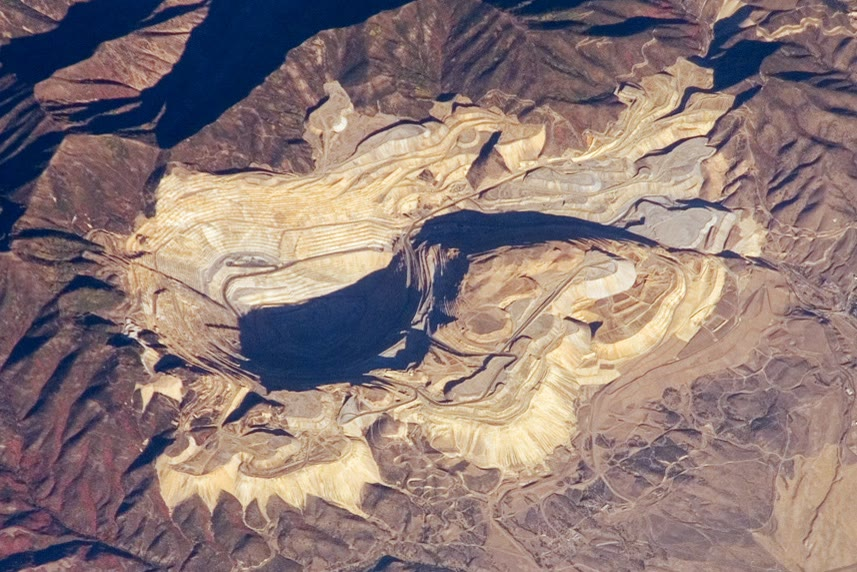
\includegraphics[width=0.5\linewidth]{images/book4/b2-29-bingham-canyon-iss.jpg}
\par\smallskip{\small The Bingham Canyon open pit, Utah, from the International Space Station
(2007): more than \qty{4}{km} wide and \qty{1200}{m} deep, cut in benches 16 to \qty{25}{m} high
into a \omterm{def:b2:ore-deposits:hydrothermal}{porphyry copper deposit}; the flat-topped hills around it are waste rock. Photograph:
NASA, Expedition 15 crew (public domain).}
\end{omfigure}
% ledger: photo:b2-29-bingham

\begin{definition}[Ore-deposit types]\label{def:b2:ore-deposits:types}
An \emph{ore-deposit type}\index{ore-deposit type} is a class of deposits that share a geological
setting, a host rock, a form, an ore mineralogy and a forming process, so that a description of
the class predicts where its members occur. The types fall into four families by process:
magmatic (the metal is concentrated by a \omterm{def:b2:magma-emplacement:magma}{magma} as it crystallises or unmixes),
hydrothermal (by a hot aqueous fluid), sedimentary (by the transport and deposition
of sediment, or precipitation from water at the surface), and supergene (by weathering
of an earlier deposit).
\end{definition}

\section{Magmatic deposits}\label{sec:b2:ore-deposits:magmatic}

\textbf{Chromite in \omterm{def:b2:magmatic-differentiation:cumulate}{layered intrusions}.} Chromite, the only commercial source of chromium,
gathers in seams of massive chromitite, more than \qty{90}{\percent} chromite, in the ultramafic
lower parts of \omterm{def:b2:magmatic-differentiation:cumulate}{layered intrusions}. The intrusions are 2 to \qty{180}{km} across and up to
\qty{15}{km} thick, and the seams range from less than a centimetre to 5--\qty{8}{m}; together
they hold most of the world's chromium reserves, and the Bushveld Complex, met in
\cref{ch:b2:magmatic-differentiation}, is the only one mined for chromite today. Their origin, a
\omterm{def:b2:magmatic-differentiation:cumulate}{cumulate} layer forced into the chromite field by the mixing of \omterm{def:b2:magma-emplacement:magma}{magmas} or a change of pressure or
oxidation state, is still debated.
% ledger: usgs10e:chromite

\textbf{Nickel--copper--PGE sulfides.} A mafic or ultramafic \omterm{def:b2:magma-emplacement:magma}{magma}, produced by large degrees of
mantle melting (\qty{20}{\percent} to \qty{25}{\percent} or more, with more than 12 per cent MgO by
weight), rises undersaturated in sulfur. If it assimilates sulfur from the crust, or cools far
enough, it becomes saturated and an immiscible sulfide liquid separates in droplets. The
chalcophile metals pass into these droplets: the ratio $D$ of their concentration in the sulfide
liquid to that in the silicate liquid, the same kind of partition coefficient as between a
mineral and a melt, is $10^2$ to $10^3$ for copper and nickel and $10^3$ to $10^4$ for the
platinum-group elements. How much metal a droplet gathers then depends on how much \omterm{def:b2:magma-emplacement:magma}{magma} it meets.
% ledger: usgs10i:r-factor

\begin{proposition}[R-factor]\label{prop:b2:ore-deposits:r-factor}
Let a unit mass of sulfide liquid separate from, and reach equilibrium with, a mass $R$ of silicate
\omterm{def:b2:magma-emplacement:magma}{magma}, the \emph{R-factor}\index{R-factor}, in a closed system; let $C_L$ be the concentration of a
metal in the \omterm{def:b2:magma-emplacement:magma}{magma} before the sulfide separated, and $D$ its sulfide--silicate partition
coefficient. Then the concentration of the metal in the sulfide is
\begin{equation}
C_S = C_L\,\frac{D\,(R + 1)}{R + D} .
\label{eq:b2:ore-deposits:r-factor}
\end{equation}
For $R \gg D$, $C_S \to D\,C_L$; for $R \ll D$, $C_S \approx (R + 1)\,C_L$.
\end{proposition}

\begin{proof}
The system of mass $R + 1$ held $(R + 1)C_L$ of the metal before separation. After it, the silicate
holds $R\,C_{\mathrm{sil}}$ and the sulfide $C_S$, with $C_S = D\,C_{\mathrm{sil}}$ at equilibrium.
Conservation gives $(R + 1)C_L = R\,C_S/D + C_S = C_S\,(R + D)/D$, hence
\eqref{eq:b2:ore-deposits:r-factor}. If $R \gg D$, $(R + 1)/(R + D) \to 1$; if $R \ll D$,
$D/(R + D) \to 1$.
\end{proof}

The two limits explain why two kinds of sulfide ore exist. When $R \ll D$ the sulfide takes
almost all the metal of the \omterm{def:b2:magma-emplacement:magma}{magma} it meets and $C_S$ grows with $R$; when $R \gg D$ it is
saturated at $D\,C_L$ and more \omterm{def:b2:magma-emplacement:magma}{magma} adds nothing. Nickel and copper, with $D$ of a few hundred,
reach their ceiling at $R$ of a few hundred to a few thousand, the range of most nickel--copper
ores; platinum and palladium, with $D$ near $10^4$, keep gaining up to $R$ of \num{10000} to
\num{100000}. Ores rich in the platinum-group elements, like the Merensky Reef of the Bushveld and
some ores of Noril'sk, therefore record a small mass of sulfide washed by a very large mass of
\omterm{def:b2:magma-emplacement:magma}{magma} (exercises~\ref{exo:b2:ore-deposits:5} and~\ref{exo:b2:ore-deposits:11}).
% ledger: usgs10i:r-factor

\textbf{Kimberlites and diamonds.} Most diamonds, and almost all mined ones, formed at the base of
thick continental lithosphere, in the roots of \omterm{def:b2:precambrian-earth:craton}{cratons}; kimberlite \omterm{def:b2:magma-emplacement:magma}{magmas}, coming from depths
greater than 120 to \qty{150}{km} and rising at up to \qty{20}{m.s^{-1}}, carry them to the
surface fast enough to survive. Kimberlites erupt preferentially through thick, old lithosphere,
which is where diamond exploration looks.
% ledger: grabreck22:kimberlite

\textbf{Pegmatites.} Lithium--cesium--tantalum pegmatites are granitic \omterm{def:b2:magma-emplacement:bodies}{dykes} enriched in these rare
elements, produced in collisional \omterm{def:b2:alpine-orogen:orogen}{orogens}; they crystallise at about 350 to \qty{550}{\celsius},
remarkably low for a granitic melt, in days to years, and grow enormous crystals --- one
spodumene crystal was \qty{14}{m} long. Their lithium minerals, spodumene, petalite and
lepidolite, supply about a quarter of the world's lithium.
% ledger: usgs10o:lct

\section{Hydrothermal deposits}\label{sec:b2:ore-deposits:hydrothermal}

\begin{definition}[Hydrothermal fluid and hydrothermal deposit types]\label{def:b2:ore-deposits:hydrothermal}
A \emph{hydrothermal fluid}\index{hydrothermal fluid} is a hot aqueous fluid, released by a \omterm{def:b2:magma-emplacement:magma}{magma},
by \omterm{def:b2:metamorphic-facies:reaction}{metamorphic reactions}, or heated sea water, meteoric water or basin brine, that dissolves,
transports and deposits elements as it flows through rock. The main hydrothermal \omterm{def:b2:ore-deposits:types}{ore-deposit types}
are:
\begin{itemize}
  \item the \emph{porphyry copper deposit}\index{porphyry copper deposit}: a large, low-grade body
        of veinlets and disseminated copper sulfides in and around a small porphyry stock, formed by
        magmatic fluids within a few kilometres of the surface above a subduction zone;
  \item the \emph{epithermal deposit}\index{epithermal deposit}: gold--silver veins and
        disseminations formed within about \qty{1.5}{km} of the surface, at about 100 to
        \qty{300}{\celsius}, in volcanic arcs;
  \item the \emph{volcanogenic massive sulfide deposit}\index{volcanogenic massive sulfide deposit}
        (VMS): a lens of massive sulfides formed on or just below the sea floor, at a hydrothermal
        vent in a submarine volcanic setting;
  \item the \emph{sedimentary exhalative deposit}\index{sedimentary exhalative deposit} (sedex):
        laminated zinc--lead sulfides in marine shales of a \omterm{def:b2:basins-compared:types}{rift basin}, precipitated on or just
        below the sea floor from basin brines rising along faults;
  \item the \emph{Mississippi Valley-type deposit}\index{Mississippi Valley-type deposit} (MVT):
        zinc--lead sulfides replacing platform carbonates, epigenetic and unrelated to igneous
        activity, deposited by basin brines;
  \item the \emph{orogenic gold deposit}\index{orogenic gold deposit}: gold-bearing quartz veins in
        metamorphic belts, along major faults, deposited by low-salinity, CO$_2$-rich fluids of
        metamorphic origin.
\end{itemize}
\end{definition}
% ledger: usgs10b:form, usgs10q:epithermal, usgs10c:vms, usgs10n:sedex, usgs10a:mvt, drew03:orogenic

\textbf{Transport and deposition.} Most metals are carried in \omterm{def:b2:ore-deposits:hydrothermal}{hydrothermal fluids} as complexes:
zinc, lead and copper as chloride complexes, so that salinity controls their solubility, and gold,
in reduced fluids, as sulfur complexes such as AuHS(H$_2$S)$_3$. A fluid drops its load when the
solubility falls: when it cools; when it boils as its pressure drops, losing H$_2$S and CO$_2$ and
changing pH; when it mixes with a fluid of different composition --- a brine meeting water rich
in H$_2$S precipitates sphalerite and galena almost at once; and when it reacts with the wall
rock, which changes its pH or oxidation state. Each deposit type is one combination of fluid,
pathway and trap.
% ledger: usgs10n:sedex, drew03:orogenic

\textbf{Porphyry copper.} Porphyry deposits supply about \qty{60}{\percent} of the world's
copper and hold about \qty{65}{\percent} of its resources. They are centred on small cylindrical
stocks or swarms of \omterm{def:b2:magma-emplacement:bodies}{dykes}, the tops of larger \omterm{def:b2:magma-emplacement:bodies}{plutons}, emplaced less than 5--\qty{10}{km} deep in
arcs above subduction zones, the setting of \cref{ch:b2:magmatic-series}. A deposit is 0.1 to
\qty{1}{km} across, with a similar height; altered rock may extend \qty{10}{km} or more around it.
As the \omterm{def:b2:magma-emplacement:magma}{magma} crystallises, a fluid with 3 to 5 per cent salt by weight separates from it; rising and
decompressing, it splits into a brine and a vapour, both carrying metals, and its overpressure
fractures the rock. Quartz veins precipitate at about 700 to \qty{500}{\celsius}, and the
reaction of the fluid with the rock zones the alteration, as in the section below. Because they
form shallow at active margins, where erosion is fast, more than \qty{90}{\percent} of known
porphyry deposits are Cenozoic or Mesozoic.
% ledger: usgs10b:share, usgs10b:form, usgs10b:fluids, usgs10b:alteration

\begin{omfigure}
\centering
\begin{tikzpicture}[x=1.15cm, y=1.15cm, font=\small]
\begin{scope}
\clip (-2.9,-3.6) rectangle (2.9,0);
% propylitic halo
\fill[omLithBasalt!45] (0,-1.25) ellipse (2.45 and 1.55);
% sodic-calcic deep flanks
\fill[omExo!25] (-1.75,-2.55) ellipse (0.45 and 0.38);
\fill[omExo!25] (1.75,-2.55) ellipse (0.45 and 0.38);
% sericitic shell
\fill[yellow!35] (0,-1.05) ellipse (1.15 and 1.15);
% potassic core
\fill[omProp!40] (0,-1.45) ellipse (0.68 and 0.85);
% ore shell
\draw[omThm, line width=1.1pt, densely dashed] (0,-1.3) ellipse (0.92 and 0.98);
% advanced argillic lithocap
\fill[omDef!30] (-1.05,0) .. controls (-0.6,-0.5) and (0.6,-0.5) .. (1.05,0) -- cycle;
\draw[omDef!70] (-1.05,0) .. controls (-0.6,-0.5) and (0.6,-0.5) .. (1.05,0);
\end{scope}
% pluton and stock
\fill[omLithGranite] (-2.6,-3.6) .. controls (-2.2,-2.9) and (-0.9,-2.6) .. (-0.3,-2.6)
  -- (-0.3,-1.25) arc[start angle=180, end angle=0, radius=0.3] -- (0.3,-2.6)
  .. controls (0.9,-2.6) and (2.2,-2.9) .. (2.6,-3.6) -- cycle;
\draw[black!60] (-2.6,-3.6) .. controls (-2.2,-2.9) and (-0.9,-2.6) .. (-0.3,-2.6)
  -- (-0.3,-1.25) arc[start angle=180, end angle=0, radius=0.3] -- (0.3,-2.6)
  .. controls (0.9,-2.6) and (2.2,-2.9) .. (2.6,-3.6);
% epithermal veins
\foreach \x in {1.45,1.65,1.85} \draw[omDef, line width=1pt] (\x,-0.02) -- (\x+0.12,-0.7);
% palaeosurface
\draw[black, line width=0.8pt] (-2.9,0) -- (2.9,0);
\node[anchor=south west, font=\scriptsize] at (-2.9,0) {palaeosurface};
% labels
\draw[black!50] (0.6,-0.15) -- (1.2,0.25) -- (3.0,0.25) node[anchor=west, text=black] {advanced argillic};
\draw[black!50] (1.95,-0.3) -- (3.0,-0.3) node[anchor=west, text=black] {epithermal veins};
\draw[black!50] (1.05,-0.8) -- (3.0,-0.8) node[anchor=west, text=black] {sericitic};
\draw[black!50] (0.85,-1.25) -- (3.0,-1.25) node[anchor=west, text=omThm] {copper ore shell};
\draw[black!50] (0.45,-1.7) -- (3.0,-1.7) node[anchor=west, text=black] {potassic};
\draw[black!50] (1.05,-2.15) -- (3.0,-2.15) node[anchor=west, text=black] {propylitic};
\draw[black!50] (2.1,-2.6) -- (3.0,-2.6) node[anchor=west, text=black] {sodic--calcic};
\draw[black!50] (1.5,-3.15) -- (3.0,-3.15) node[anchor=west, text=black] {pluton and porphyry stock};
\end{tikzpicture}
\par\smallskip{\small A porphyry copper system in section (a drawing, not to scale): the potassic
zone in the core, deep and hot; the sericitic zone upward and outward, where pyrite is
abundant; the copper ore shell between them; the propylitic halo at shallow to moderate depths
around; sodic--calcic alteration on the deep flanks; an advanced argillic cap and, in some
systems, epithermal veins near the surface.}
\end{omfigure}
% ledger: usgs10b:alteration

\textbf{Epithermal gold.} Above some porphyry systems, and in volcanic arcs generally, the same
kind of fluids reach the upper \qty{1.5}{km} of the crust at about 100 to \qty{300}{\celsius},
where they boil and mix with ground water; they deposit gold and silver in quartz veins, with
alteration that records near-neutral fluids (adularia, illite) or very acid ones (kaolinite,
dickite, pyrophyllite).
% ledger: usgs10q:epithermal, usgs10q:alteration

\textbf{Massive sulfides on the sea floor.} Sea water drawn down into the hot crust of a ridge or
an arc returns at vents as black smokers at about \qty{350}{\celsius}, first seen on the East
Pacific Rise in 1979. Where the vent field lasts, its sulfides build a mound; the ore is more than
\qty{40}{\percent} sulfides, over a stockwork of veins that marks the feeder. The metals are zoned
by temperature, iron and copper at the hot base, zinc, iron, lead and barium at the cooler top and
margins, as in the mound drawn in the next section. \omterm{def:b2:ore-deposits:hydrothermal}{Volcanogenic massive sulfide
deposits} range from pods of less than a tonne to the \qty{1.5}{Gt} of Rio Tinto in Spain, and in
age from \qty{3.55}{\Ga} to deposits forming today.
% ledger: usgs10c:vms

\textbf{Basin brines: sedex and MVT.} Basin brines of 10 to \qty{30}{\percent} dissolved salts,
heated to 100--\qty{200}{\celsius} by burial, carry zinc and lead as chloride complexes and form the
two sediment-hosted types. Sedex deposits form where the brine vents into a restricted, reduced
basin along a rift fault and meets hydrogen sulfide, making laminated sulfide muds; they hold more
than half of the world's zinc and lead reserves. MVT deposits form where the brine, driven out of a
basin, reaches a carbonate platform at its margin and replaces it at 75 to about
\qty{200}{\celsius}; they hold \qty{38}{\percent} of the lead and zinc of the sediment-hosted
deposits, with about ten times more zinc than lead.
% ledger: usgs10n:sedex, usgs10a:mvt

\textbf{Orogenic gold.} In metamorphic belts, \omterm{def:b2:metamorphic-facies:reaction}{devolatilisation reactions} release a near-neutral,
low-salinity fluid rich in CO$_2$; channelled along major faults, it deposits gold-bearing quartz
veins at about \qty{350}{\celsius} and 4 to \qty{12}{km} depth. The veins are continuous over
great heights: \qty{3.2}{km} at Kolar, in India.
% ledger: drew03:orogenic

\section{Sedimentary and supergene deposits}\label{sec:b2:ore-deposits:sedimentary}

\begin{definition}[Placer]\label{def:b2:ore-deposits:placer}
A \emph{placer}\index{placer} is a sedimentary deposit of dense, durable minerals concentrated by
moving water or wind because, for the same size, they settle faster and are entrained less easily
than the quartz grains around them.
\end{definition}

Minerals denser than about 2.85 are called heavy, against 2.65 for quartz: ilmenite and zircon
near 4.7, magnetite 5.2, gold 15 to 19.3. By Stokes's law a grain's settling velocity grows with
its excess density $\rho_s - \rho_w$, eleven times larger for gold than for quartz, so gold of a
given size sits with quartz three times as large (exercise~\ref{exo:b2:ore-deposits:3}); gold
usually stays in river gravels on bedrock, while ilmenite, rutile and zircon reach beaches and
dunes. Grades in heavy-mineral sands are the weight per cent of heavy minerals.
% ledger: usgs10l:heavy, usgs:gold-placer

Chemical sediments are ores too. The \omterm{def:b2:precambrian-earth:bif}{banded iron formations} of \cref{ch:b2:precambrian-earth},
precipitated as the oceans' dissolved iron was oxidised, are a common ore of iron; evaporites
supply halite and the potassium salts; laterites, the residue of deep tropical weathering,
concentrate aluminium as bauxite. Weathering also upgrades earlier deposits.
% ledger: earle:bif, usgs:bauxite

\begin{definition}[Supergene enrichment, gossan]\label{def:b2:ore-deposits:supergene}
\emph{Supergene enrichment}\index{supergene enrichment} is the concentration of a metal by
descending ground water: above the water table, oxygenated, acid water dissolves the metal from the
sulfides of an orebody, and below it, in reducing conditions, deposits it again, mostly by
replacing the primary sulfides. A \emph{gossan}\index{gossan} is the porous, iron-oxide rich rock
left at the surface over a weathered sulfide body, its sulfides replaced by goethite, hematite and
jarosite.
\end{definition}

In porphyry deposits, the leached capping above the water table is up to several hundred metres
thick; below it, enriched sulfide zones of chalcocite, tens to several hundred metres thick, reach
more than \qty{1.5}{Gt} at 0.4 to \qty{1.7}{\percent} copper, always richer than the primary,
hypogene ore beneath. The iron oxides of a \omterm{def:b2:ore-deposits:supergene}{gossan} and of a leached capping keep the textures of the
sulfides they replaced, and guide the search below; \omterm{def:b2:ore-deposits:supergene}{gossans} and their iron staining revealed many
massive sulfide deposits to early miners.
% ledger: usgs10b:supergene, usgs10c:vms

\begin{omfigure}
\centering
\begin{minipage}[b]{0.46\linewidth}\centering
\begin{tikzpicture}[x=1cm, y=1cm, font=\scriptsize]
\fill[omHist!55] (0,4.0) rectangle (1.8,5.2);
\fill[omMeth!30] (0,3.0) rectangle (1.8,4.0);
\fill[black!55] (0,1.8) rectangle (1.8,3.0);
\fill[black!18] (0,0) rectangle (1.8,1.8);
\draw (0,0) rectangle (1.8,5.2);
\draw[omDef, line width=1pt, densely dashed] (-0.25,3.0) -- (2.05,3.0);
\foreach \x in {0.45,0.9,1.35} \draw[omDef, -{Stealth[length=4pt]}] (\x,5.0) -- (\x,3.2);
\node[anchor=west, align=left] at (2.0,4.6) {gossan and leached\\capping (Fe oxides)};
\node[anchor=west, align=left] at (2.0,3.5) {oxide zone\\(malachite)};
\node[anchor=east, text=omDef, align=right] at (-0.25,3.0) {water\\table};
\node[anchor=west, align=left] at (2.0,2.4) {enrichment blanket\\(chalcocite)};
\node[anchor=west, align=left] at (2.0,0.9) {primary ore\\(chalcopyrite\\+ pyrite)};
\node[anchor=south, font=\scriptsize, text=omDef] at (0.9,5.25) {acid water, Cu$^{2+}$};
\end{tikzpicture}
\end{minipage}\hfill
\begin{minipage}[b]{0.52\linewidth}\centering
\begin{tikzpicture}[x=1cm, y=1cm, font=\scriptsize]
\fill[omSea] (-2.6,1.4) rectangle (2.6,3.2);
\fill[omLithBasalt!60] (-2.6,-1.6) rectangle (2.6,1.4);
% stockwork cone
\fill[omProp!25] (-0.5,-1.6) -- (0.5,-1.6) -- (1.1,0.9) -- (-1.1,0.9) -- cycle;
\foreach \x/\y in {-0.3/-1.2,0.1/-1.0,-0.6/-0.4,0.4/-0.3,-0.1/0.1,0.6/0.4,-0.7/0.5}
  \draw[omProp!80!black] (\x,\y) -- ++(0.35,0.25);
% mound: upper rim and core
\fill[yellow!45] (-1.8,1.4) .. controls (-1.2,2.35) and (1.2,2.35) .. (1.8,1.4) -- cycle;
\fill[omThm!45] (-1.1,1.4) .. controls (-0.7,2.0) and (0.7,2.0) .. (1.1,1.4) -- cycle;
\draw (-1.8,1.4) .. controls (-1.2,2.35) and (1.2,2.35) .. (1.8,1.4);
% chimney and plume
\fill[black!70] (-0.08,2.1) rectangle (0.08,2.55);
\fill[black!45] (0,2.6) circle (0.12) (0.1,2.8) circle (0.16) (0.25,3.0) circle (0.2);
\draw[omDef, -{Stealth[length=4pt]}] (-2.3,2.9) -- (-2.3,0.2) -- (-1.2,-0.9);
\draw[omThm, -{Stealth[length=4pt]}] (0,-1.5) -- (0,1.2);
\node[anchor=west, text=omDef] at (-2.55,3.05) {sea water};
\node[anchor=west] at (0.45,2.85) {black smoker, \qty{350}{\celsius}};
\draw[black!50] (1.45,1.75) -- (2.0,2.15) node[anchor=west, text=black] {Zn, Fe, Pb, Ba};
\draw[black!50] (0.6,1.6) -- (2.0,1.15) node[anchor=west, text=black] {Fe, Cu};
\node[anchor=west, align=left] at (0.95,-0.4) {stockwork\\(feeder)};
\node[anchor=north, text=omThm] at (0,-1.6) {hot fluid};
\end{tikzpicture}
\end{minipage}
\par\smallskip{\small Left: a supergene profile over a copper sulfide body (a drawing, not to
scale): acid water leaches copper above the water table and redeposits it as chalcocite below,
leaving a \omterm{def:b2:ore-deposits:supergene}{gossan} at the surface. Right: a volcanogenic massive sulfide mound in section (a
drawing): sea water heated in the crust rises through a stockwork and vents as a black smoker; the
mound is zoned from iron and copper at the hot base to zinc, iron, lead and barium at the top and
margins.}
\end{omfigure}
% ledger: usgs10b:supergene, usgs10c:vms

\begin{omfigure}
\centering
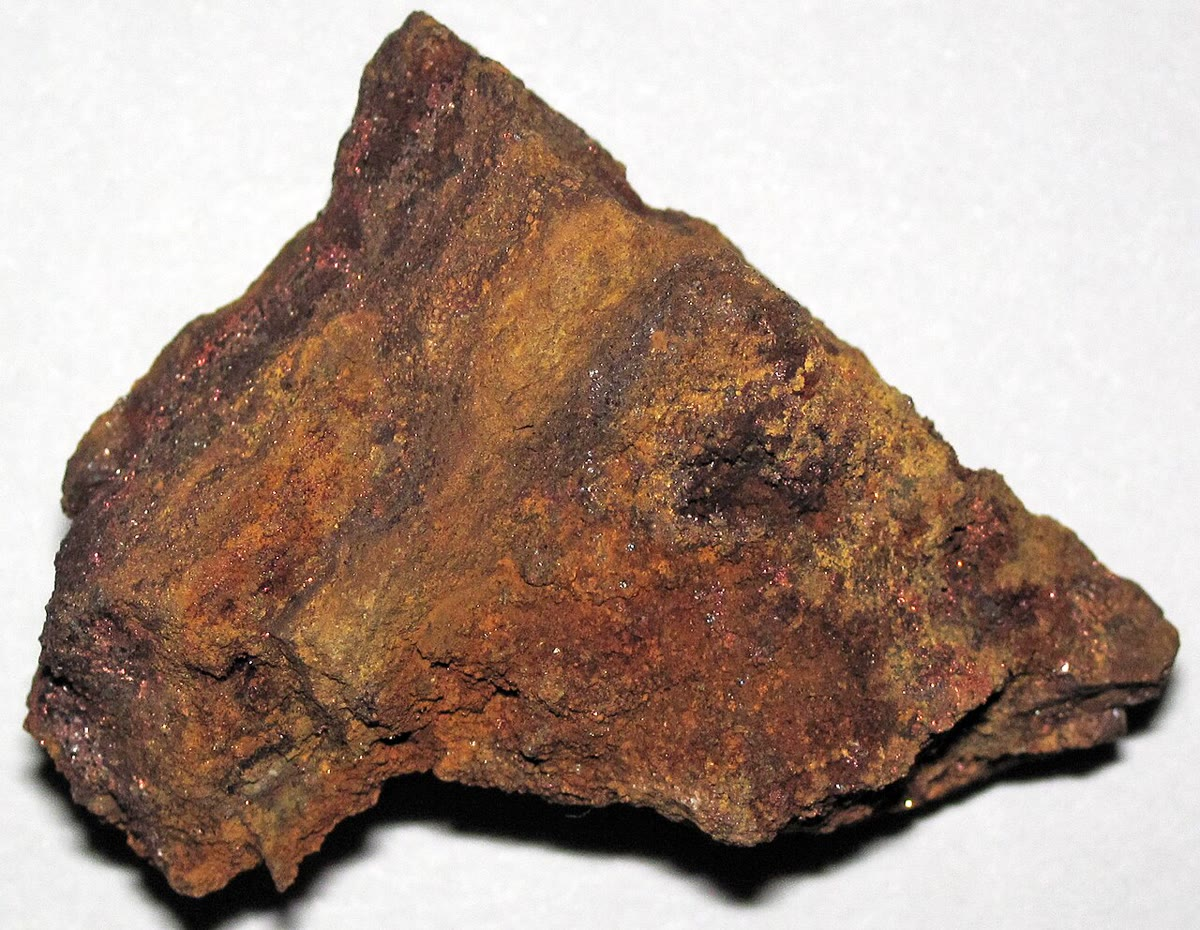
\includegraphics[width=0.4\linewidth]{images/book4/b2-29-flambeau-gossan.jpg}
\par\smallskip{\small \omterm{def:b2:ore-deposits:supergene}{Gossan} from the Flambeau massive sulfide deposit, Wisconsin: a porous rock of
iron hydroxy-oxides left by the weathering of pyrite, chalcopyrite, chalcocite and bornite in a
Palaeoproterozoic volcanic arc; the small orange specks are native copper. Photograph: James St.
John (CC BY 2.0).}
\end{omfigure}
% ledger: photo:b2-29-gossan

\section{Grade and tonnage}\label{sec:b2:ore-deposits:grade-tonnage}

A world compilation lists 422 \omterm{def:b2:ore-deposits:hydrothermal}{porphyry copper deposits} with their \omterm{def:b2:ore-deposits:grade}{tonnage}, at the lowest available
cut-off, and their mean copper grade. A tenth of them exceed \qty{1500}{Mt} and a tenth hold less
than \qty{33}{Mt}, with a median of \qty{240}{Mt}; the grades run from \qty{0.24}{\percent} to
\qty{0.75}{\percent} between the same deciles, with a median of \qty{0.44}{\percent}. Between the
deciles the \omterm{def:b2:ore-deposits:grade}{tonnage} spreads over a factor of 45, the grade over a factor of 3. On logarithmic axes both histograms are close to normal curves, as the figure below shows:
the logarithms of \omterm{def:b2:ore-deposits:grade}{tonnage} have a mean of 2.373 and a standard deviation of 0.654, those of grade
$-0.364$ and 0.199 (logarithms to base 10, \omterm{def:b2:ore-deposits:grade}{tonnage} in megatonnes, grade in per cent). The fit is
imperfect: the grades are more peaked than a log-normal law, and a few very low-grade deposits make
them depart from it in a formal test. And the two are almost independent, with a correlation of
0.1 between their logarithms.
% ledger: usgs08:table1, usgs08:independence, data:b4-porphyry-cu

\begin{omfigure}
\centering
\begin{minipage}[b]{0.49\linewidth}\centering
\begin{tikzpicture}
\begin{axis}[omrecord, width=0.96\linewidth, height=4.5cm, xmin=0.5, xmax=5.0, ymin=0, ymax=80,
  xlabel={tonnage (Mt)}, ylabel={number of deposits},
  xtick={1,2,3,4,5}, xticklabels={10,100,1000,$10^4$,$10^5$},
  tick label style={font=\scriptsize}, label style={font=\small}]
% computed in figdata/bachelor-2/ores.py part hist_t; ledger: data:b4-porphyry-cu
\addplot[ybar, bar width=0.22, fill=omDef!35, draw=omDef!70] table[x=log10_t, y=count] {figdata/out/bachelor-2-ores-hist_t.dat};
\addplot[omThm, line width=1pt, smooth] table[x=log10_t, y=fit] {figdata/out/bachelor-2-ores-hist_t.dat};
\end{axis}
\end{tikzpicture}
\end{minipage}\hfill
\begin{minipage}[b]{0.49\linewidth}\centering
\begin{tikzpicture}
\begin{axis}[omrecord, width=0.96\linewidth, height=4.5cm, xmin=-1.2, xmax=0.6, ymin=0, ymax=120,
  xlabel={copper grade (\%)}, ylabel={number of deposits},
  xtick={-1,-0.69897,-0.30103,0,0.30103}, xticklabels={0.1,0.2,0.5,1,2},
  tick label style={font=\scriptsize}, label style={font=\small}]
% computed in figdata/bachelor-2/ores.py part hist_g; ledger: data:b4-porphyry-cu
\addplot[ybar, bar width=0.088, fill=omDef!35, draw=omDef!70] table[x=log10_g, y=count] {figdata/out/bachelor-2-ores-hist_g.dat};
\addplot[omThm, line width=1pt, smooth] table[x=log10_g, y=fit] {figdata/out/bachelor-2-ores-hist_g.dat};
\end{axis}
\end{tikzpicture}
\end{minipage}
\par\smallskip{\small The \omterm{def:b2:ore-deposits:grade}{tonnage} (left) and the copper grade (right) of the 422 \omterm{def:b2:ore-deposits:hydrothermal}{porphyry copper
deposits} of the world compilation, on logarithmic axes, with the normal curves of the same mean
and standard deviation in red. Data: Singer, Berger and Moring (2008), USGS.}
\end{omfigure}

\begin{proposition}[Product of log-normal variables]\label{prop:b2:ore-deposits:product}
If $\log_{10} T$ and $\log_{10} g$ are jointly normal, with means $\mu_T$ and $\mu_g$, standard
deviations $\sigma_T$ and $\sigma_g$ and correlation $\rho$, then the contained metal $M = Tg/100$
($g$ in per cent) is log-normal: $\log_{10} M$ is normal with
\begin{equation}
\mu_M = \mu_T + \mu_g - 2 , \qquad
\sigma_M^2 = \sigma_T^2 + \sigma_g^2 + 2\rho\,\sigma_T\sigma_g .
\label{eq:b2:ore-deposits:product}
\end{equation}
\end{proposition}

\begin{proof}
$\log_{10} M = \log_{10} T + \log_{10} g - 2$. A linear combination of jointly normal variables is
normal (admitted from the mathematics books); its mean is the sum of the means and its variance
$\operatorname{var}(X + Y) = \operatorname{var} X + \operatorname{var} Y + 2\operatorname{cov}(X, Y)$,
with $\operatorname{cov}(X, Y) = \rho\,\sigma_T\sigma_g$.
\end{proof}

For the porphyry deposits, $\sigma_M = \sqrt{0.654^2 + 0.199^2 + 2 \times 0.1 \times 0.654 \times
0.199} = 0.702$ and $\mu_M = 0.009$: the median deposit holds about \qty{1}{Mt} of copper, and the
contained metal spreads even more widely than the \omterm{def:b2:ore-deposits:grade}{tonnage}. A log-normal law with so wide a spread
puts most of the metal in a few deposits: the largest tenth hold about \qty{63}{\percent} of the
copper by the law, \qty{64}{\percent} in the data (exercise~\ref{exo:b2:ore-deposits:12}). The
figure below plots each deposit by its \omterm{def:b2:ore-deposits:grade}{tonnage} and grade, with lines of equal contained copper;
Bingham, at \qty{28.5}{Mt}, lies between the 10 and \qty{100}{Mt} lines.
% ledger: data:b4-porphyry-cu
% values: sd_log10_m 0.702233, mean 0.00857; median M 1.02 Mt; top 10 % share 0.631 (fit) 0.643 (data)

\begin{definition}[Grade--tonnage curve]\label{def:b2:ore-deposits:gt}
The \emph{grade--tonnage curve}\index{grade--tonnage curve} of a deposit gives, as functions of
the \omterm{def:b2:ore-deposits:grade}{cut-off grade} $c$, the \omterm{def:b2:ore-deposits:grade}{tonnage} $T(c)$ of the blocks with a grade above $c$ and their mean grade
$\bar g(c)$.
\end{definition}

\begin{proposition}[Grade--tonnage curve of a log-normal deposit]\label{prop:b2:ore-deposits:gt}
If the grades of the blocks of a deposit of total \omterm{def:b2:ore-deposits:grade}{tonnage} $T_0$ are log-normal, $\ln g$ normal
with mean $\mu$ (the median grade is $e^{\mu}$) and standard deviation $s$, then, with $z = (\mu -
\ln c)/s$,
\begin{equation}
T(c) = T_0\,\Phi(z), \qquad
\bar g(c) = e^{\mu + s^2/2}\,\frac{\Phi(z + s)}{\Phi(z)} ,
\label{eq:b2:ore-deposits:gt}
\end{equation}
and the metal above the cut-off is $M(c) = T_0\,e^{\mu + s^2/2}\,\Phi(z + s)$, a fraction $\Phi(z +
s)$ of the whole.
\end{proposition}

\begin{proof}
Write $\ln g = \mu + s u$, with $u$ standard normal. A block is above the cut-off when $u > (\ln c -
\mu)/s = -z$, which has probability $1 - \Phi(-z) = \Phi(z)$; hence $T(c)$. The metal above the
cut-off per unit of total \omterm{def:b2:ore-deposits:grade}{tonnage} is $\int_{-z}^{\infty} e^{\mu + s u}\,\varphi(u)\,\mathrm{d}u$,
with $\varphi$ the standard normal density. Completing the square, $e^{su}\varphi(u) =
e^{s^2/2}\varphi(u - s)$, so the integral is $e^{\mu + s^2/2}\,[1 - \Phi(-z - s)] = e^{\mu +
s^2/2}\,\Phi(z + s)$. Dividing by $\Phi(z)$ gives the mean grade.
\end{proof}

At $c \to 0$ the whole deposit is kept, at the mean grade $e^{\mu + s^2/2}$, which is above the
median. Raising the cut-off removes \omterm{def:b2:ore-deposits:grade}{tonnage} faster than metal, because the blocks removed are the
poorest: in the illustrative deposit of the figure, raising the cut-off from 0.2 to
\qty{0.5}{\percent} keeps \qty{41}{\percent} of the \omterm{def:b2:ore-deposits:grade}{tonnage} but \qty{61}{\percent} of the copper.
% values: demo T 876.0/355.0 Mt, M 4.599/2.826 Mt (figdata ores.py gtcurve)

\begin{omfigure}
\centering
\begin{minipage}[b]{0.49\linewidth}\centering
\begin{tikzpicture}
\begin{axis}[omrecord, width=0.96\linewidth, height=5.0cm, xmode=log, ymode=log,
  xmin=2, xmax=50000, ymin=0.05, ymax=2.8, xlabel={tonnage (Mt)}, ylabel={copper grade (\%)},
  ytick={0.1,0.2,0.5,1,2}, yticklabels={0.1,0.2,0.5,1,2},
  tick label style={font=\scriptsize}, label style={font=\small}]
% computed in figdata/bachelor-2/ores.py parts scatter and iso; ledger: data:b4-porphyry-cu
\addplot[black!45, line width=0.6pt, unbounded coords=jump] table[x=tonnage_mt, y=g01] {figdata/out/bachelor-2-ores-iso.dat};
\addplot[black!45, line width=0.6pt, unbounded coords=jump] table[x=tonnage_mt, y=g1] {figdata/out/bachelor-2-ores-iso.dat};
\addplot[black!45, line width=0.6pt, unbounded coords=jump] table[x=tonnage_mt, y=g10] {figdata/out/bachelor-2-ores-iso.dat};
\addplot[black!45, line width=0.6pt, unbounded coords=jump] table[x=tonnage_mt, y=g100] {figdata/out/bachelor-2-ores-iso.dat};
\addplot[omDef, only marks, mark=*, mark size=0.8pt, opacity=0.7] table[x=tonnage_mt, y=cu_pct] {figdata/out/bachelor-2-ores-scatter.dat};
\addplot[omThm, only marks, mark=square*, mark size=2pt] coordinates {(3230,0.882)};
\node[font=\tiny, text=black!70, fill=white, inner sep=1pt] at (axis cs:4.55,2.2) {0.1};
\node[font=\tiny, text=black!70, fill=white, inner sep=1pt] at (axis cs:45.5,2.2) {1};
\node[font=\tiny, text=black!70, fill=white, inner sep=1pt] at (axis cs:455,2.2) {10};
\node[font=\tiny, text=black!70, fill=white, inner sep=1pt] at (axis cs:4545,2.2) {100 Mt};
\node[font=\scriptsize, text=omThm, anchor=south, fill=white, inner sep=1pt] at (axis cs:3230,1.0) {Bingham};
\end{axis}
\end{tikzpicture}
\end{minipage}\hfill
\begin{minipage}[b]{0.49\linewidth}\centering
\begin{tikzpicture}
\begin{axis}[omrecord, width=0.80\linewidth, height=5.0cm, xmin=0, xmax=1.2, ymin=0, ymax=1000,
  xlabel={cut-off grade (\%)}, ylabel={tonnage above cut-off (Mt)}, axis y line*=left,
  ylabel style={text=omDef}, tick label style={font=\scriptsize}, label style={font=\small}]
% computed in figdata/bachelor-2/ores.py part gtcurve (illustrative deposit)
\addplot[omDef, line width=1.1pt] table[x=cutoff_pct, y=tonnage_mt] {figdata/out/bachelor-2-ores-gtcurve.dat};
\end{axis}
\begin{axis}[width=0.80\linewidth, height=5.0cm, xmin=0, xmax=1.2, ymin=0, ymax=1.6,
  axis y line*=right, axis x line=none, ylabel={mean grade above cut-off (\%)},
  ylabel style={text=omThm}, tick label style={font=\scriptsize}, label style={font=\small}]
\addplot[omThm, line width=1.1pt, densely dashed] table[x=cutoff_pct, y=grade_pct] {figdata/out/bachelor-2-ores-gtcurve.dat};
\end{axis}
\end{tikzpicture}
\end{minipage}
\par\smallskip{\small Left: \omterm{def:b2:ore-deposits:grade}{tonnage} and copper grade of the 422 \omterm{def:b2:ore-deposits:hydrothermal}{porphyry copper deposits}, with
lines of equal contained copper (0.1 to \qty{100}{Mt}); the red square is Bingham Canyon. Data:
Singer, Berger and Moring (2008), USGS. Right: the \omterm{def:b2:ore-deposits:gt}{grade--tonnage curve} of an illustrative deposit
of \qty{1000}{Mt}, median grade \qty{0.40}{\percent}, $s = 0.60$: \omterm{def:b2:ore-deposits:grade}{tonnage} above the cut-off (blue)
and its mean grade (red, dashed), from \eqref{eq:b2:ore-deposits:gt}.}
\end{omfigure}

\section{Exploration}\label{sec:b2:ore-deposits:exploration}

Deposits are found by the traces they leave beyond their ore. The alteration halo of a porphyry
system is kilometres wide, and where the rock is exposed its minerals can be mapped from aircraft
and satellites by their infrared spectra; its metals disperse into the soils, stream sediments, waters and plants around
it; and its sulfides and altered rocks change the physical properties that geophysics measures.
% ledger: usgs10b:form, usgs10b:exploration, usgs10b:remote

\begin{definition}[Geochemical anomaly]\label{def:b2:ore-deposits:exploration}
A \emph{geochemical anomaly}\index{geochemical anomaly} is a concentration of an element, or of a
group of elements, in a sampled medium --- rock, soil, stream sediment, water, plants --- that
departs from its background in the region, the range of concentrations found where no
mineralisation is present.
\end{definition}

Like grades, concentrations spread over orders of magnitude, so an anomaly is usually judged on
logarithms; one simple threshold, used in exercise~\ref{exo:b2:ore-deposits:9}, is the mean of
the logarithms of the background plus twice their standard deviation. A stream sediment sample
mixes the sediment of its whole catchment, so an anomaly fades downstream as clean sediment joins
it, and the gradient of the concentrations points up the drainage toward the source. In soils over
buried pegmatites, anomalies of lithium, rubidium, cesium, tantalum and tin have been traced above
bodies that do not crop out.
% ledger: usgs10b:exploration, usgs10o:lct

Geophysical methods are chosen for the contrast a deposit type offers. Disseminated sulfides make a
rock act as a capacitor: the induced polarisation method, which measures this chargeability, was
developed for porphyry copper and responds most to the pyrite-rich sericitic zone, the potassic
core being poorer in sulfides. Magnetic and gravity surveys map the \omterm{def:b2:magma-emplacement:bodies}{plutons} to which the deposits
are related. No method sees ore
directly, and every interpretation is non-unique until a drill hole tests it.
% ledger: usgs10b:exploration

\begin{method}[From assays to a resource estimate]\label{met:b2:ore-deposits:resource}
The data are drill holes on a grid across the deposit, their core logged and assayed in intervals
of known length.
\begin{enumerate}
  \item \textbf{Composite.} Average the assays over equal lengths, weighting each assay by its
        length, so that every composite represents the same volume.
  \item \textbf{Model.} Divide the deposit into blocks and estimate the grade of each from the
        nearby composites, weighting them by distance and by the spatial correlation of the grades
        (the geostatistical method of kriging, admitted).
  \item \textbf{Report.} Apply a cut-off: \omterm{def:b2:ore-deposits:grade}{tonnage} and mean grade of the blocks above it, with the
        density of the rock, at each confidence level allowed by the drill spacing.
\end{enumerate}
\end{method}

\begin{inthefield}[Logging drill core]
\centering
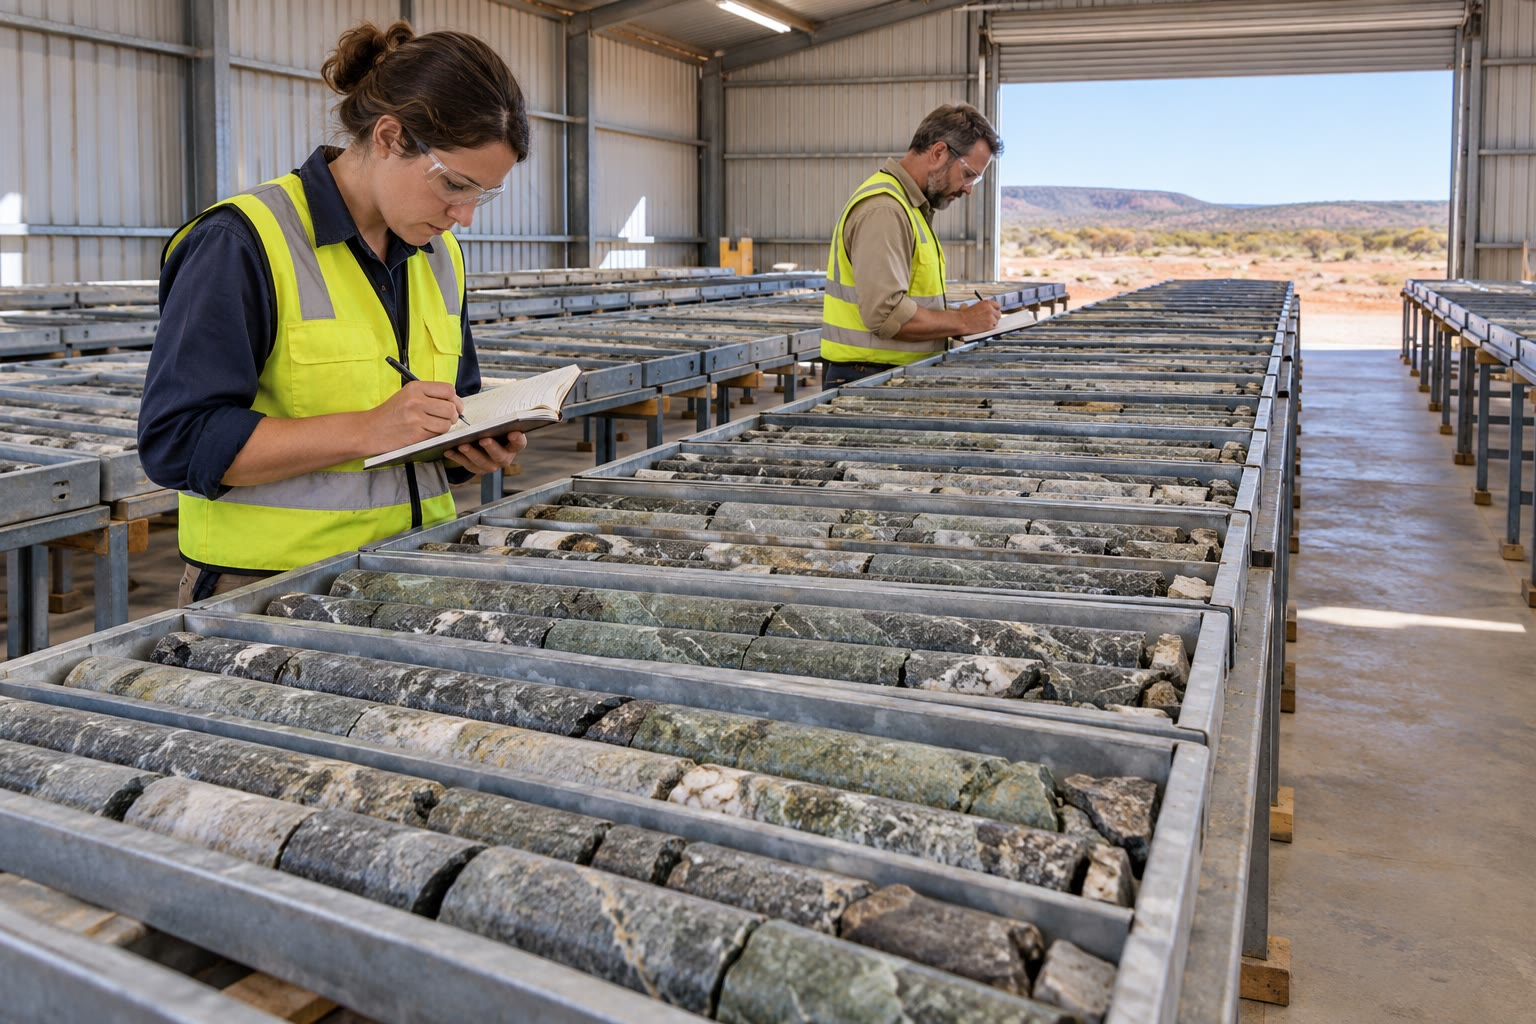
\includegraphics[width=0.56\linewidth]{images/book4/ai/b2-core-shed.jpg}
\par\smallskip{\small A core shed at an exploration project (AI-generated illustration).}
\par\medskip\raggedright
On an exploration project, the core from each drill hole is laid out in metal trays in the order
it came out of the ground. Geologists walk the trays, interval by interval, and record what the
rock is, how it is altered, which veins cut it and in what proportion, and which sulfides it
holds; they mark where the core will be sawn and sampled. The log comes before the assays and is
compared with them: an alteration zone or a vein type that carries the metal becomes the thing to
follow from hole to hole, and from the log the geologists draw the sections from which the next
holes are planned.
\end{inthefield}

\section*{Exercises}\label{sec:b2:ore-deposits:exercises}

Data for the exercises, unless stated otherwise: upper continental crust, copper \qty{28}{ppm},
gold \qty{1.5}{ng/g}, chromium \qty{92}{ppm}; the porphyry copper population of
\cref{sec:b2:ore-deposits:grade-tonnage}, $\log_{10}$ \omterm{def:b2:ore-deposits:grade}{tonnage} (Mt) mean 2.373 and standard
deviation 0.654, $\log_{10}$ grade (\%) mean $-0.364$ and standard deviation 0.199, correlation
$\rho = 0.100$. Round to three significant figures.
% ledger: rg03:ucc-trace, data:b4-porphyry-cu

\begin{exercise}[$\star$]\label{exo:b2:ore-deposits:1}
Find the \omterm{def:b2:ore-deposits:cf}{concentration factor} against the upper crust of: (a) a copper ore at
\qty{0.5}{\percent}; (b) a gold ore at \qty{6}{g/t}; (c) a chromitite of \qty{90}{\percent}
chromite, taking chromite as FeCr$_2$O$_4$ (atomic masses Cr 52.00, Fe 55.85, O 16.00).
\end{exercise}

\begin{exercise}[$\star$]\label{exo:b2:ore-deposits:2}
Batu Hijau is reported as \qty{914}{Mt} at \qty{0.53}{\percent} Cu and \qty{0.40}{g/t} Au above a
\qty{0.3}{\percent} cut-off, and as \qty{1640}{Mt} at \qty{0.44}{\percent} Cu and \qty{0.45}{g/t}
Au at the lowest available cut-off. (a) Find the contained copper (Mt) and gold (t) of each
estimate. (b) What \omterm{def:b2:ore-deposits:grade}{tonnage} and what copper do the extra blocks of the second estimate add, and at
what mean grade? (c) Why are both estimates correct?
\end{exercise}

\begin{exercise}[$\star$]\label{exo:b2:ore-deposits:3}
In Stokes's law the settling velocity of a grain of diameter $d$ is proportional to $(\rho_s -
\rho_w)\,d^2$. Take $\rho_w = 1.00$, quartz 2.65, gold 19.3, zircon 4.7 (in
\unit{g.cm^{-3}}). (a) How many times faster does a gold grain settle than a quartz grain of the
same size? (b) What is the ratio of the diameters of a gold and a quartz grain that settle at the
same speed? (c) Which quartz grain settles like a zircon grain of \qty{0.1}{mm}?
\end{exercise}

\begin{exercise}[$\star$]\label{exo:b2:ore-deposits:4}
A primary copper ore has a grade of \qty{0.4}{\percent}. Weathering leaches all its copper over a
thickness of \qty{150}{m} and redeposits it in a blanket \qty{50}{m} thick just below, the density
being the same. (a) Find the grade of the blanket. (b) The same if only \qty{80}{\percent} of the
leached copper is redeposited. (c) What leached thickness would give \qty{1.7}{\percent} with
complete redeposition?
\end{exercise}

\begin{exercise}[$\star\star$]\label{exo:b2:ore-deposits:5}
A \omterm{def:b2:magma-emplacement:magma}{magma} holds \qty{10}{ppb} of platinum and \qty{200}{ppm} of nickel; take $D_{\mathrm{Pt}} =
10^4$ and $D_{\mathrm{Ni}} = 500$. (a) Using \eqref{eq:b2:ore-deposits:r-factor}, find the
platinum (ppm) and nickel (wt\%) contents of the sulfide for $R = 100$, \num{1000}, \num{10000}
and \num{100000}. (b) Find their limits for $R \to \infty$. (c) Explain why a nickel ore says
little about $R$, and a platinum ore much.
\end{exercise}

\begin{exercise}[$\star\star$]\label{exo:b2:ore-deposits:6}
Using \eqref{eq:b2:ore-deposits:product} for the porphyry copper population: (a) find the mean and
standard deviation of $\log_{10} M$, and the median contained copper. (b) What fraction of deposits
holds more than \qty{10}{Mt} of copper? How many of 422? (c) Repeat (b) ignoring the correlation.
\end{exercise}

\begin{exercise}[$\star\star$]\label{exo:b2:ore-deposits:7}
For the illustrative deposit of the figure ($T_0 = \qty{1000}{Mt}$, median \qty{0.40}{\percent},
$s = 0.60$), use \eqref{eq:b2:ore-deposits:gt} to find the \omterm{def:b2:ore-deposits:grade}{tonnage}, mean grade and contained copper
above cut-offs of \qty{0.3}{\percent} and \qty{0.6}{\percent}. Check one point on the figure.
\end{exercise}

\begin{exercise}[$\star\star$]\label{exo:b2:ore-deposits:8}
A porphyry deposit holds \qty{5}{Mt} of copper. Suppose its magmatic fluid carried \qty{1000}{ppm}
of copper, half of which was deposited in the ore, and that the \omterm{def:b2:magma-emplacement:magma}{magma} released \qty{3.5}{\percent}
of its mass as fluid. (a) Find the mass of fluid and of \omterm{def:b2:magma-emplacement:magma}{magma} needed. (b) Find the volume of the
\omterm{def:b2:magma-emplacement:magma}{magma}, of density \qty{2600}{kg.m^{-3}}. (c) If the \omterm{def:b2:magma-emplacement:magma}{magma} held \qty{50}{ppm} copper, what fraction
of it ended in the ore?
\end{exercise}

\begin{exercise}[$\star\star$]\label{exo:b2:ore-deposits:9}
Eight background stream sediments give $\log_{10}$ Cu (ppm) of 1.30, 1.45, 1.38, 1.52, 1.41, 1.35,
1.48 and 1.40. (a) Find the mean and standard deviation (population) of the logarithms, the
background median and the threshold mean plus two standard deviations, in ppm. (b) A tributary
draining \qty{4}{km^2} of mineralised ground carries sediment at \qty{400}{ppm}; it joins a stream
draining \qty{36}{km^2} at the background median. Assuming each square kilometre yields the same
mass of sediment, is the mixed sediment anomalous? (c) Up to what total catchment area does the
anomaly stay above the threshold?
\end{exercise}

\begin{exercise}[$\star\star\star$]\label{exo:b2:ore-deposits:10}
(a) Prove $e^{su}\varphi(u) = e^{s^2/2}\varphi(u - s)$. (b) Deduce the mean of a log-normal
variable, $e^{\mu + s^2/2}$. (c) Show that the fraction of the metal above the cut-off,
$\Phi(z + s)$, always exceeds the fraction of the \omterm{def:b2:ore-deposits:grade}{tonnage}, $\Phi(z)$, and interpret.
\end{exercise}

\begin{exercise}[$\star\star\star$]\label{exo:b2:ore-deposits:11}
(a) From \eqref{eq:b2:ore-deposits:r-factor}, find the $R$ at which $C_S$ reaches a fraction $f$
of its ceiling $D\,C_L$. (b) Evaluate it for $f = 0.5$ and $0.9$ with $D = 300$ (nickel) and $D =
10^4$ (platinum). (c) Compare with the ranges of $R$ of nickel--copper ores and of PGE reefs given
in the text.
\end{exercise}

\begin{exercise}[$\star\star\star$]\label{exo:b2:ore-deposits:12}
(a) For a log-normal variable $M$ with $\ln M$ of standard deviation $s$, show that the deposits above
the quantile of order $q$ hold a fraction $\Phi\bigl(s - \Phi^{-1}(q)\bigr)$ of the total metal.
(b) Evaluate it for the porphyry population and $q = 0.9$. (c) The same for $q = 0.99$; compare with
the four largest deposits, which hold \qty{26.6}{\percent} of the copper of the compilation.
\end{exercise}
% ledger: data:b4-porphyry-cu

\begin{problem}[{Weekend problem --- A porphyry prospect}]\label{pb:b2:ore-deposits:1}
A porphyry prospect (invented) has been drilled. Its discovery hole cut eight intervals, from top
to bottom (length in metres, copper grade in per cent): 30 m at 0.12; 40 at 0.35; 50 at 0.62; 60
at 0.48; 40 at 0.27; 30 at 0.81; 50 at 0.41; 30 at 0.18. A geostatistical study of all the holes
finds that the block grades are log-normal, with median \qty{0.38}{\percent} and $s = 0.55$ for
$\ln g$. The mineralised body is close to a vertical cylinder of radius \qty{450}{m} and height
\qty{700}{m}, of density \qty{2.7}{t.m^{-3}}. Use the data of the exercises, and round to three
significant figures (probabilities to four).

\noindent\textbf{Part I --- The discovery hole.}
\begin{enumerate}
  \item Find the length of the hole sampled and its length-weighted mean grade.
  \item Find the arithmetic mean of the eight grades. Why is the weighted mean the right one?
  \item Which fraction of the length is above \qty{0.3}{\percent}, and at what mean grade?
  \item Find the \omterm{def:b2:ore-deposits:cf}{concentration factor} of the weighted mean grade against the upper crust.
  \item The same for the richest interval.
  \item Find the mean grade of all the blocks of the deposit. Is the discovery hole representative?
\end{enumerate}

\noindent\textbf{Part II --- Tonnage above the cut-off.}
\begin{enumerate}[resume]
  \item Find the volume and the \omterm{def:b2:ore-deposits:grade}{tonnage} $T_0$ of the body; keep $T_0 = \qty{1200}{Mt}$.
  \item For a cut-off of \qty{0.3}{\percent}, find $z$ and the fraction of the blocks above it.
  \item Find the \omterm{def:b2:ore-deposits:grade}{tonnage} above cut-offs of 0.2, 0.3 and \qty{0.5}{\percent}.
  \item Find the mean grade above the \qty{0.3}{\percent} cut-off.
  \item The same above 0.2 and \qty{0.5}{\percent}.
  \item Raising the cut-off from 0.3 to \qty{0.5}{\percent}: by what factors do the \omterm{def:b2:ore-deposits:grade}{tonnage} and the
        mean grade change?
  \item At which cut-off is half the \omterm{def:b2:ore-deposits:grade}{tonnage} kept, and what is its mean grade?
\end{enumerate}

\noindent\textbf{Part III --- The prospect among the world's porphyries.}
\begin{enumerate}[resume]
  \item Find the copper contained in the whole body, at its mean grade.
  \item Find the standard score of its \omterm{def:b2:ore-deposits:grade}{tonnage} in the world population, and its percentile.
  \item The same for its mean grade.
  \item Find the standard deviation of $\log_{10} M$ with the correlation, and without it.
  \item Find the percentile of its contained copper.
  \item How many of the 422 deposits would be expected to hold more copper?
\end{enumerate}

\noindent\textbf{Part IV --- Copper above the cut-off.}
\begin{enumerate}[resume]
  \item Find the copper contained above the \qty{0.2}{\percent} cut-off.
  \item The same above \qty{0.5}{\percent}.
  \item What fraction of the copper lies above \qty{0.3}{\percent}, and what fraction of the
        \omterm{def:b2:ore-deposits:grade}{tonnage}?
  \item Explain why lowering the cut-off below \qty{0.3}{\percent} adds much rock and little
        copper, using the answers to questions 9 and 20.
  \item To sum up: how much copper does the prospect contain above the \qty{0.3}{\percent} cut-off?
\end{enumerate}
\end{problem}
